\documentclass{article}

\usepackage{graphicx}
\usepackage{tikz}
\usepackage{tikzsymbols}
\usetikzlibrary{calc,patterns,shapes.geometric}
\pagestyle{empty}
\usepackage[margin=0pt]{geometry}
\geometry{papersize={14in,12in}}

\def\centerarc[#1](#2)(#3:#4:#5){\draw[#1] ($(#2)+({#5*cos(#3)},{#5*sin(#3)})$) arc (#3:#4:#5);}

\begin{document}
	\begin{figure}
		\centering
		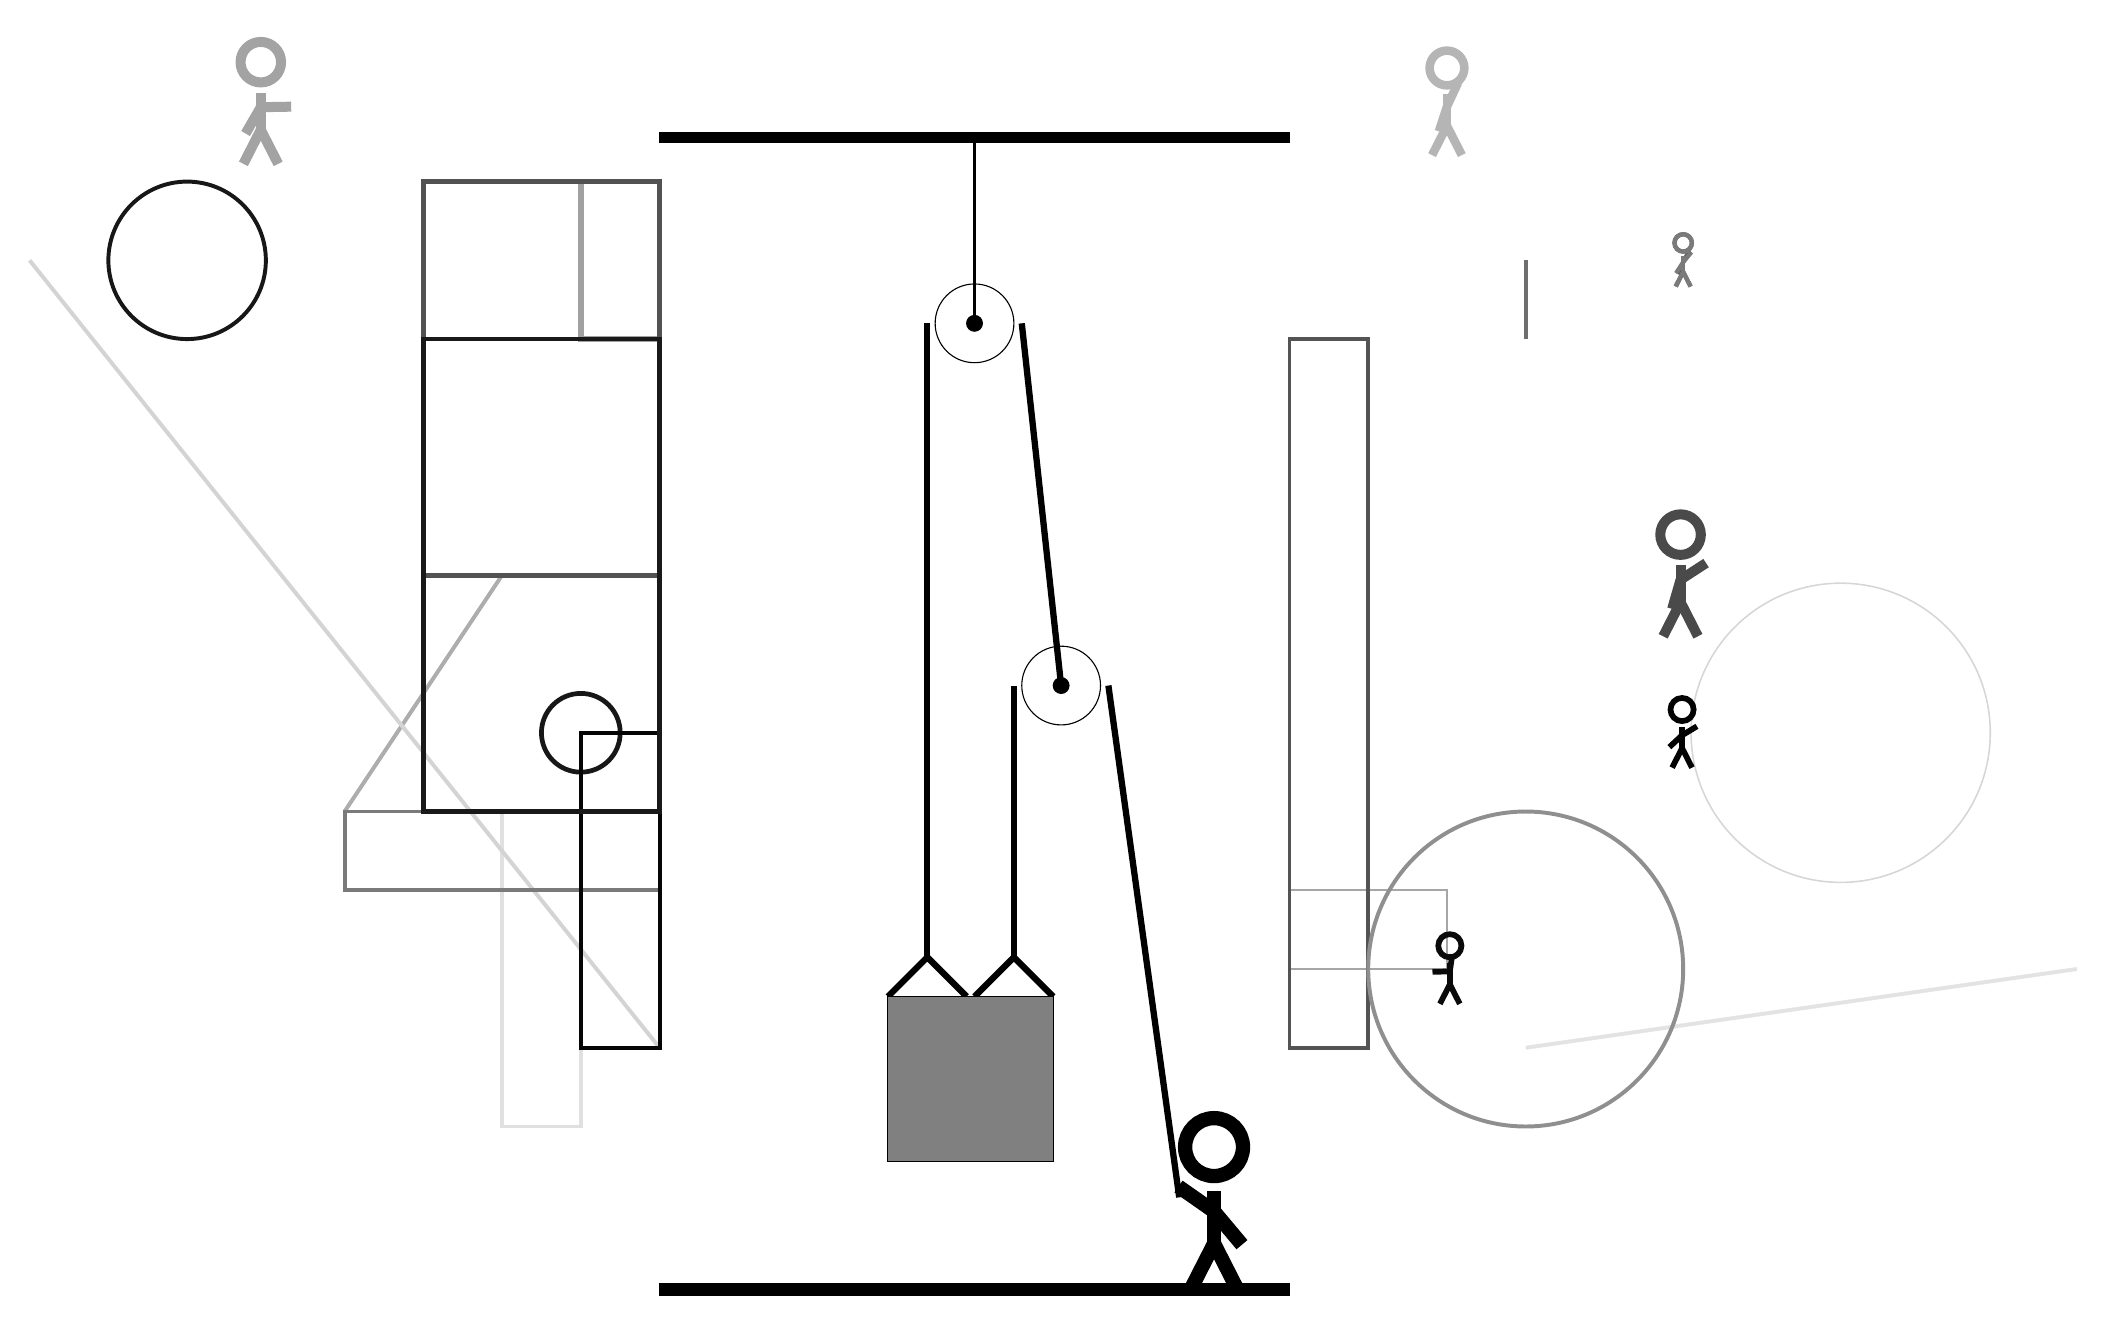
\begin{tikzpicture}
			%%%%% START %%%%%
			
			\draw[fill=black] (-2, 11.5) rectangle (6, 11.625);
			
			\draw (2, 9.2) circle (0.5);
			\draw[fill=black] (2, 9.2) circle (0.1);
			\draw[thick] (2, 9.2) -- (2, 11.5);
			
			\draw (3.1, 4.6) circle (0.5);
			\draw[fill=black] (3.1, 4.6) circle (0.1);
			
			\draw [line width=0.6mm, color=black!91](-3, 4) circle (0.5);
			
			\draw [line width=0.4mm, color=black!24](9, 1) circle (0.0);
			\node[line width=0.2mm, color=black!63] at (11, 10) {\Strichmaxerl[3][65][62]};
			\draw[line width=0.7mm, color=black!37] (-3, 9) rectangle (-2, 11);
			\draw[line width=0.5mm, color=black!12] (-3, -1) rectangle (-4, 3);
			
			\draw[line width=0.2mm, color=black!35] (8, 1) rectangle (6, 2);
			\draw [line width=0.5mm, color=black!86](11, 4) circle (0.0);
			\draw[line width=0.5mm, color=black!67] (6, 0) rectangle (7, 9);
			\draw[line width=0.5mm, color=black!32](-4, 6) -- (-6, 3);
			\draw[line width=0.6mm, color=black!68] (-2, 6) rectangle (-5, 11);
			
			\draw [line width=0.5mm, color=black!91](-8, 10) circle (1.0);
			
			\draw[line width=0.5mm, color=black!17](-2, 0) -- (-10, 10);
			\node[line width=0.4mm, color=black!52] at (11, 10) {\Strichmaxerl[3][57][51]};
			
			\draw[line width=0.5mm, color=black!11](9, 0) -- (16, 1);
			\draw[line width=0.5mm, color=black!52] (-2, 3) rectangle (-6, 2);
			\node[line width=0.3mm, color=black!29] at (8, 12) {\Strichmaxerl[6][72][65]};
			
			\node[line width=0.2mm, color=black!96] at (8, 1) {\Strichmaxerl[4][1][82]};
			
			\node[line width=0.6mm, color=black!36] at (-7, 12) {\Strichmaxerl[7][60][1]};
			\node[line width=0.5mm, color=black!71] at (11, 6) {\Strichmaxerl[7][74][33]};
			
			\draw[line width=0.5mm, color=black!57](9, 10) -- (9, 9);
			\draw [line width=0.2mm, color=black!16](13, 4) circle (1.9);
			
			\draw [line width=0.5mm, color=black!44](9, 1) circle (2.0);
			\node[line width=0.7mm, color=black!99] at (11, 4) {\Strichmaxerl[4][43][31]};
			\draw[line width=0.5mm, color=black!98] (-2, 4) rectangle (-3, 0);
			\draw[line width=0.6mm, color=black!90] (-2, 9) rectangle (-5, 3);
			
			
			\draw[line width = 0.8mm]  (0.9, 0.65) -- (1.4, 1.15) -- (1.9, 0.65);
			\draw[line width = 0.8mm]  (2.0, 0.65) -- (2.5, 1.15) -- (3.0, 0.65);
			\draw[fill=black!50] (0.9, 0.65) rectangle (3.0, -1.45);
			
			\draw[line width = 0.8mm] (1.4, 9.2) -- (1.4, 1.15);
			\centerarc[line width = 0.8mm](2, 9.2)(0:180:0.6);
			\draw[line width = 0.8mm] (2.6, 9.2) -- (3.1, 4.6);
			\draw[line width = 0.8mm] (2.5, 4.6) -- (2.5, 1.15);
			\centerarc[line width = 0.8mm](3.1, 4.6)(0:180:0.6);
			\draw[line width = 0.8mm] (3.7, 4.6) -- (4.6, -1.9);
			
			\node at (5, -2) {\Strichmaxerl[10][-35][-50]};
			
			\draw[fill=black] (-2, -3) rectangle (6, -3.15);
			
			%%%%% END %%%%%
		\end{tikzpicture}
	\end{figure}	
\end{document}